% ============================================================
% LAPORAN PRAKTIKUM ALGORITMA DAN PEMROGRAMAN
% Modul 1: Variabel, Tipe Data, dan Struktur Kontrol Percabangan
% Compile dengan pdfLaTeX
% ============================================================

\documentclass[12pt,a4paper]{article}

% ---------- Font sederhana ----------
\usepackage[T1]{fontenc}
\usepackage[utf8]{inputenc}
\usepackage{mathptmx}

% ---------- Tata letak ----------
\usepackage[a4paper,left=3cm,right=2cm,top=2cm,bottom=2cm]{geometry}
\usepackage{setspace}
\setstretch{1.15}
\usepackage{ragged2e}
\justifying
\setlength{\parindent}{1.25cm}
\setlength{\parskip}{0pt}

% ---------- Paket umum ----------
\usepackage{graphicx}
\usepackage{float}
\usepackage{enumitem}
\usepackage{titlesec}
\usepackage{array}
\usepackage{booktabs}
\usepackage{longtable}
\usepackage{caption}
\usepackage{hyperref}
\usepackage{amsmath}
\hypersetup{hidelinks}

% ---------- Format heading ----------
\titleformat{\section}
  {\bfseries\fontsize{12pt}{14pt}\selectfont}
  {}{0pt}{}
\titlespacing*{\section}{0pt}{12pt}{6pt}

\titleformat{\subsection}
  {\bfseries\fontsize{12pt}{14pt}\selectfont}
  {}{0pt}{}
\titlespacing*{\subsection}{0pt}{10pt}{4pt}

\titleformat{\subsubsection}
  {\bfseries\fontsize{12pt}{14pt}\selectfont}
  {}{0pt}{}
\titlespacing*{\subsubsection}{0pt}{8pt}{3pt}

\setlist[enumerate]{leftmargin=1.1cm,itemsep=0pt,topsep=2pt}
\setlist[itemize]{leftmargin=1.1cm,itemsep=0pt,topsep=2pt}

% ---------- Helper template ----------
\newcommand{\placeholder}[1]{\textit{[#1]}}
\newcommand{\imageplaceholder}[1]{%
  \begin{center}
  \fbox{\parbox[c][5.5cm][c]{0.88\textwidth}{\centering\textit{[#1]}}}
  \end{center}
}

\begin{document}

% ============================================================
% COVER
% ============================================================
\begin{titlepage}
\thispagestyle{empty}
\begin{center}

{\bfseries\fontsize{16pt}{19pt}\selectfont LAPORAN PRAKTIKUM\par}
\vspace{0.25cm}
{\bfseries\fontsize{16pt}{19pt}\selectfont ALGORITMA DAN PEMROGRAMAN\par}
\vspace{0.45cm}
{\bfseries\fontsize{14pt}{17pt}\selectfont MODUL 1\par}
\vspace{0.15cm}
{\bfseries\fontsize{14pt}{17pt}\selectfont VARIABEL, TIPE DATA, DAN STRUKTUR KONTROL PERCABANGAN\par}

\vspace{1.2cm}

\IfFileExists{logo_telkom_university.png}{%
  
\includegraphics[width=0.34\textwidth]{logo_telkom_university.png}%
}{%
  \IfFileExists{../logo_telkom_university.png}{%
    \includegraphics[width=0.34\textwidth]{../logo_telkom_university.png}%
  }{%
    \IfFileExists{../../logo_telkom_university.png}{%
      
\includegraphics[width=0.34\textwidth]{../../logo_telkom_university.png}%
    }{%
      \fbox{\parbox[c][3.5cm][c]{0.34\textwidth}{\centering\textit{[Logo Telkom University]}}}%
    }%
  }%
}

\vspace{1.2cm}

\renewcommand{\arraystretch}{1.35}
\begin{tabular}{>{\bfseries}p{2.3cm} p{0.35cm} p{8.4cm}}
NAMA  & : & DENDRA DE TAMA \\
NIM   & : & 108052600034 \\
KELAS & : & SS1SI-50-REG-01 \\
PRODI & : & S1 SISTEM INFORMASI \\
\end{tabular}

\vfill

{\bfseries TELKOM UNIVERSITY SURABAYA\par}
{\bfseries FAKULTAS REKAYASA INDUSTRI\par}
{\bfseries PROGRAM STUDI S1 SISTEM INFORMASI\par}
\vspace{0.2cm}
{\bfseries TAHUN AKADEMIK 2025/2026\par}

\end{center}
\end{titlepage}

% ============================================================
% PENDAHULUAN
% ============================================================
\section{PENDAHULUAN}
Pemrograman komputer pada dasarnya adalah proses penyusunan serangkaian instruksi terstruktur untuk memproses data menjadi informasi yang berguna. Dalam bahasa pemrograman Python, variabel berfungsi sebagai lokasi penyimpanan bernama di dalam memori komputer yang digunakan untuk menampung nilai data tertentu sehingga dapat dipanggil dan diolah kembali pada tahapan komputasi selanjutnya. Python mengadopsi mekanisme pengetikan dinamis (\textit{dynamic typing}), di mana deklarasi tipe data tidak perlu dituliskan secara eksplisit, melainkan ditentukan secara otomatis pada saat pemberian nilai awal (\textit{variable assignment}) melalui operator sama dengan ($=$). Penamaan variabel diwajibkan mengikuti kaidah baku, yakni hanya memuat karakter alfanumerik dan garis bawah (\textit{underscore}), diawali oleh huruf atau garis bawah, bersifat sensitif terhadap huruf kapital (\textit{case-sensitive}), serta dianjurkan menerapkan gaya penulisan \textit{snake\_case}.

Setiap data di dalam Python diklasifikasikan ke dalam tipe data dasar tertentu yang menentukan operasi apa saja yang dapat dilakukan terhadapnya. Tipe data dasar yang paling esensial meliputi bilangan bulat (\texttt{int}), bilangan riil berpresisi desimal (\texttt{float}), barisan karakter teks (\texttt{str}), serta nilai kebenaran logika (\texttt{bool}). Python tidak memiliki tipe data karakter tunggal terpisah (\texttt{char}); karakter individual tetap direpresentasikan sebagai string dengan panjang satu. Untuk memeriksa klasifikasi tipe data dari suatu variabel, Python menyediakan fungsi bawaan \texttt{type()}.

Selain penyimpanan data statis, interaktivitas program dibangun melalui fungsi masukan dan keluaran (\textit{input/output}). Fungsi \texttt{input()} digunakan untuk menangkap teks masukan dari pengguna melalui konsol. Karena keluaran murni fungsi \texttt{input()} selalu bertipe \texttt{str}, konversi tipe data eksplisit (\textit{type casting}) menggunakan fungsi konversi seperti \texttt{int()} atau \texttt{float()} mutlak diperlukan sebelum data numerik dioperasikan secara matematis.

Pengambilan keputusan di dalam algoritma diatur oleh struktur kontrol percabangan. Percabangan memungkinkan program menentukan cabang alur eksekusi mana yang akan dijalankan berdasarkan evaluasi kondisi logika (\textit{Boolean expression}). Dalam Python, struktur percabangan diimplementasikan melalui kata kunci \texttt{if}, \texttt{elif}, dan \texttt{else}. Python tidak menggunakan kurung kurawal (\texttt{\{\}}) untuk membatasi blok perintah, melainkan mengandalkan indentasi spasi (\textit{indentation}) yang konsisten. Kondisi percabangan dievaluasi menggunakan operator relasional komparasi ($==$, $!=$, $>$, $<$, $\ge$, $\le$) dan operasi aritmatika pembantu seperti modulo ($\%$) untuk mendeteksi paritas bilangan.

Praktikum Modul 1 ini mencakup empat latihan terbimbing serta satu studi kasus komprehensif, meliputi deklarasi variabel multi-tipe dan inspeksi tipe data (\texttt{latihan1.py}), pembacaan masukan dan manipulasi aritmatika (\texttt{latihan2.py}), percabangan biner klasifikasi paritas ganjil/genap (\texttt{latihan3.py}), percabangan berantai kategori nilai ujian (\texttt{latihan4.py}), serta penentuan status kelulusan akademik mahasiswa beserta konversi grade huruf mutu (\texttt{studi\_kasus.py}).

\subsection{Tujuan Praktikum}
\begin{enumerate}
    \item Memahami konsep deklarasi variabel, alokasi memori dinamis, serta aturan penamaan \textit{snake\_case} pada Python 3.
    \item Mengidentifikasi dan membedakan tipe data dasar (\texttt{str}, \texttt{int}, \texttt{float}, \texttt{bool}) serta memeriksa tipe variabel menggunakan fungsi intrinsik \texttt{type()}.
    \item Mengimplementasikan operasi pembacaan masukan pengguna via \texttt{input()} dan melakukan konversi tipe eksplisit (\textit{type casting}) untuk operasi aritmatika.
    \item Menerapkan struktur kontrol percabangan biner (\texttt{if-else}) dan percabangan multi-kondisi (\texttt{if-elif-else}) dengan aturan indentasi Python.
    \item Merancang dan mengimplementasikan logika penentuan status kelulusan mahasiswa serta konversi grade huruf pada studi kasus akademik.
\end{enumerate}

% ============================================================
% LANGKAH PERCOBAAN
% ============================================================
\section{LANGKAH--LANGKAH PERCOBAAN}

\subsection{Percobaan 1: Deklarasi Variabel dan Tipe Data (latihan1.py)}
\begin{enumerate}
    \item Pemahaman Persoalan: Program bertujuan untuk mendemonstrasikan pendefinisian variabel dengan empat tipe data primitif yang berbeda (\texttt{str}, \texttt{int}, \texttt{float}, dan \texttt{bool}) serta memverifikasi kelas tipe data dari masing-masing variabel menggunakan fungsi bawaan \texttt{type()}.
    \item Data Masukan/Keluaran:
    \begin{itemize}
        \item Masukan: Tidak ada masukan dinamis dari pengguna (nilai diinisialisasi secara statis pada kode sumber).
        \item Keluaran: Nilai keempat variabel yang dicetak dalam satu baris, diikuti empat baris keluaran kelas tipe data objek (\texttt{<class 'str'>}, \texttt{<class 'int'>}, \texttt{<class 'float'>}, dan \texttt{<class 'bool'>}).
    \end{itemize}
    \item Penyusunan Algoritma:
    \begin{enumerate}[label=\alph*.]
        \item Mulai program.
        \item Inisialisasi variabel string \texttt{nama} dengan nilai \texttt{"Aurora"}.
        \item Inisialisasi variabel integer \texttt{umur} dengan nilai \texttt{21}.
        \item Inisialisasi variabel float \texttt{tinggi\_badan} dengan nilai \texttt{165.0}.
        \item Inisialisasi variabel boolean \texttt{adalah\_mahasiswa} dengan nilai \texttt{True}.
        \item Tampilkan nilai keempat variabel secara berdampingan.
        \item Tampilkan hasil evaluasi \texttt{type(nama)}, \texttt{type(umur)}, \texttt{type(tinggi\_badan)}, dan \texttt{type(adalah\_mahasiswa)}.
        \item Selesai.
    \end{enumerate}
\end{enumerate}

\subsection{Percobaan 2: Input dari Pengguna dan Konversi Tipe (latihan2.py)}
\begin{enumerate}
    \item Pemahaman Persoalan: Program berfungsi untuk membaca data tekstual dan data numerik dari papan ketik melalui fungsi \texttt{input()}. Masukan umur harus dikonversi dari string ke integer menggunakan \texttt{int()} agar dapat diproses oleh operasi aritmatika penambahan satu tahun untuk proyeksi umur tahun depan.
    \item Data Masukan/Keluaran:
    \begin{itemize}
        \item Masukan: Teks \texttt{nama} bertipe string dan angka \texttt{umur} bertipe numerik.
        \item Keluaran: Kalimat sapaan nama pengguna serta kalimat proyeksi usia pengguna di tahun depan.
    \end{itemize}
    \item Penyusunan Algoritma:
    \begin{enumerate}[label=\alph*.]
        \item Mulai program.
        \item Tampilkan prompt dan baca string masukan pengguna ke variabel \texttt{nama}.
        \item Tampilkan prompt, baca string masukan usia, dan konversikan secara eksplisit ke integer ke dalam variabel \texttt{umur}.
        \item Tampilkan teks sapaan \texttt{"Halo, "} diikuti nilai variabel \texttt{nama}.
        \item Hitung ekspresi $umur + 1$ dan tampilkan kalimat proyeksi usia tahun depan.
        \item Selesai.
    \end{enumerate}
\end{enumerate}

\subsection{Percobaan 3: Percabangan if-else Bilangan Ganjil/Genap (latihan3.py)}
\begin{enumerate}
    \item Pemahaman Persoalan: Program menguji paritas bilangan bulat masukan pengguna. Bilangan genap didefinisikan secara matematis sebagai bilangan yang habis dibagi 2 (sisa pembagian modulo bernilai nol), sedangkan bilangan ganjil menyisakan nilai 1 ketika dimodulo 2. Keputusan diambil melalui struktur kontrol percabangan biner \texttt{if-else}.
    \item Data Masukan/Keluaran:
    \begin{itemize}
        \item Masukan: Sebuah bilangan bulat (\texttt{angka}) bertipe integer.
        \item Keluaran: Informasi penegasan bahwa bilangan tersebut adalah bilangan genap atau bilangan ganjil.
    \end{itemize}
    \item Penyusunan Algoritma:
    \begin{enumerate}[label=\alph*.]
        \item Mulai program.
        \item Baca masukan bilangan integer ke dalam variabel \texttt{angka}.
        \item Evaluasi kondisi relasional: apakah $angka \pmod 2 == 0$?
        \begin{itemize}
            \item Jika bernilai \textit{True}, cetak teks bahwa angka tersebut adalah bilangan genap.
            \item Jika bernilai \textit{False}, cetak teks bahwa angka tersebut adalah bilangan ganjil.
        \end{itemize}
        \item Selesai.
    \end{enumerate}
\end{enumerate}

\subsection{Percobaan 4: Percabangan if-elif-else Kategori Nilai (latihan4.py)}
\begin{enumerate}
    \item Pemahaman Persoalan: Program dirancang untuk mengklasifikasikan nilai ujian berskala 0 hingga 100 ke dalam empat kategori mutu huruf mutu (A, B, C, D) menggunakan struktur percabangan berantai \texttt{if-elif-else}. Urutan evaluasi disusun menurun dari ambang batas tertinggi ke batas terendah.
    \item Data Masukan/Keluaran:
    \begin{itemize}
        \item Masukan: Nilai ujian (\texttt{nilai}) berupa bilangan bulat integer dalam interval 0--100.
        \item Keluaran: Kategori nilai huruf (\texttt{"A"}, \texttt{"B"}, \texttt{"C"}, atau \texttt{"D"}).
    \end{itemize}
    \item Penyusunan Algoritma:
    \begin{enumerate}[label=\alph*.]
        \item Mulai program.
        \item Baca nilai ujian pengguna ke variabel \texttt{nilai}.
        \item Uji kondisi pertama: jika $nilai \ge 85$, tetapkan $kategori = \text{"A"}$.
        \item Jika salah, uji kondisi kedua: jika $nilai \ge 70$, tetapkan $kategori = \text{"B"}$.
        \item Jika salah, uji kondisi ketiga: jika $nilai \ge 55$, tetapkan $kategori = \text{"C"}$.
        \item Jika semua kondisi salah, tetapkan $kategori = \text{"D"}$.
        \item Cetak teks \texttt{"Kategori nilai kamu: "} beserta nilai variabel \texttt{kategori}.
        \item Selesai.
    \end{enumerate}
\end{enumerate}

\subsection{Percobaan 5: Studi Kasus Cek Kelulusan Mahasiswa (studi\_kasus.py)}
\begin{enumerate}
    \item Pemahaman Persoalan: Program mengimplementasikan sistem evaluasi kelulusan akademik mahasiswa. Program menerima masukan nama mahasiswa dan nilai akhir (0--100). Berdasarkan aturan akademik, nilai $\ge 60$ dinyatakan \texttt{LULUS}, sedangkan nilai $< 60$ dinyatakan \texttt{TIDAK LULUS}. Program juga mengimplementasikan tantangan tambahan berupa penentuan grade huruf akademik (A/B/C/D) serta mencetak hasil evaluasi secara terformat rapi.
    \item Data Masukan/Keluaran:
    \begin{itemize}
        \item Masukan: Teks \texttt{nama} mahasiswa dan angka \texttt{nilai} akhir (integer).
        \item Keluaran: Kalimat status kelulusan mahasiswa (\texttt{"[nama] dengan nilai akhir [nilai] dinyatakan [status]"}) serta baris informasi \texttt{"Grade: [grade]"}.
    \end{itemize}
    \item Penyusunan Algoritma:
    \begin{enumerate}[label=\alph*.]
        \item Mulai program.
        \item Baca nama mahasiswa ke variabel string \texttt{nama}.
        \item Baca nilai akhir mahasiswa dan ubah ke integer ke variabel \texttt{nilai}.
        \item Evaluasi syarat kelulusan: jika $nilai \ge 60$, maka $status = \text{"LULUS"}$, selain itu $status = \text{"TIDAK LULUS"}$.
        \item Tampilkan kalimat status kelulusan mahasiswa.
        \item Evaluasi grade huruf:
        \begin{itemize}
            \item Jika $nilai \ge 85$, maka $grade = \text{"A"}$.
            \item Jika $nilai \ge 70$, maka $grade = \text{"B"}$.
            \item Jika $nilai \ge 55$, maka $grade = \text{"C"}$.
            \item Selain itu, $grade = \text{"D"}$.
        \end{itemize}
        \item Tampilkan teks \texttt{"Grade: "} diikuti nilai variabel \texttt{grade}.
        \item Selesai.
    \end{enumerate}
\end{enumerate}

% ============================================================
% HASIL DAN ANALISIS
% ============================================================
\section{HASIL DAN ANALISIS PERCOBAAN}

Pada bagian ini disajikan penjabaran algoritma terperinci, dokumentasi luaran eksekusi program, serta analisis komprehensif terhadap lima percobaan praktikum Python 3 pada Modul 1.

\subsection{Percobaan 1: Deklarasi Variabel dan Tipe Data}
\subsubsection{Algoritma}
\begin{enumerate}
    \item Mulai program.
    \item Alokasikan variabel \texttt{nama} dan assign nilai string \texttt{"Aurora"}.
    \item Alokasikan variabel \texttt{umur} dan assign nilai integer \texttt{21}.
    \item Alokasikan variabel \texttt{tinggi\_badan} dan assign nilai float \texttt{165.0}.
    \item Alokasikan variabel \texttt{adalah\_mahasiswa} dan assign nilai boolean \texttt{True}.
    \item Cetak nilai variabel \texttt{nama}, \texttt{umur}, \texttt{tinggi\_badan}, dan \texttt{adalah\_mahasiswa} yang dipisahkan oleh spasi.
    \item Panggil fungsi intrinsik \texttt{type()} untuk mengevaluasi tipe data dari masing-masing variabel dan tampilkan hasilnya secara berurutan.
    \item Selesai.
\end{enumerate}

\subsubsection{Hasil / Output}
\begin{figure}[H]
    \centering
    \IfFileExists{image/latihan1.png}{%
        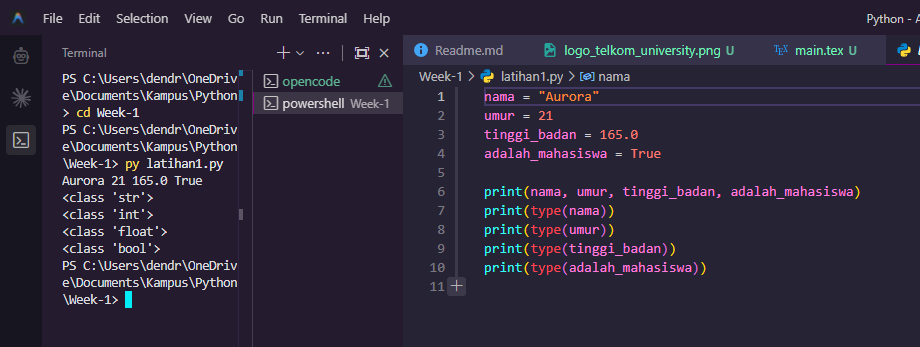
\includegraphics[width=0.85\textwidth]{image/latihan1.png}%
    }{%
        \imageplaceholder{Output Percobaan 1: Deklarasi Variabel dan Tipe Data}%
    }
    \caption{Hasil/Output Percobaan 1: Deklarasi Variabel dan Tipe Data}
\end{figure}

\subsubsection{Analisis}
Percobaan 1 mendemonstrasikan sifat \textit{dynamic typing} pada Python. Berbeda dengan bahasa berpengetikan statis seperti C atau Java yang mewajibkan deklarasi tipe sebelum variabel digunakan, interpreter Python secara implisit mengenali tipe data berdasarkan nilai literal yang diberikan. Nilai \texttt{"Aurora"} dialokasikan sebagai objek kelas \texttt{'str'}, bilangan bulat \texttt{21} sebagai \texttt{'int'}, angka berkoma \texttt{165.0} sebagai bilangan riil \texttt{'float'}, serta nilai kebenaran \texttt{True} sebagai \texttt{'bool'}.

Fungsi bawaan \texttt{type()} membuktikan bahwa setiap variabel di Python merupakan instansiasi dari kelas tertentu. Penggunaan satu perintah \texttt{print(nama, umur, tinggi\_badan, adalah\_mahasiswa)} secara otomatis menyisipkan karakter spasi sebagai pemisah bawaan (\textit{default separator}), menghasilkan keluaran yang terbaca jelas tanpa perlu konversi manual ke string.

\subsection{Percobaan 2: Input dari Pengguna dan Konversi Tipe}
\subsubsection{Algoritma}
\begin{enumerate}
    \item Mulai program.
    \item Panggil fungsi \texttt{input("Masukkan nama: ")} dan simpan hasilnya ke variabel \texttt{nama}.
    \item Panggil fungsi \texttt{input("Masukkan umur: ")}, lakukan konversi eksplisit dengan \texttt{int()}, lalu simpan hasilnya ke variabel \texttt{umur}.
    \item Tampilkan string sapaan \texttt{"Halo,"} beserta isi variabel \texttt{nama}.
    \item Hitung ekspresi penjumlahan $umur + 1$, lalu tampilkan hasilnya di antara teks \texttt{"Tahun depan usiamu"} dan \texttt{"tahun"}.
    \item Selesai.
\end{enumerate}

\subsubsection{Hasil / Output}
\begin{figure}[H]
    \centering
    \IfFileExists{image/latihan2.png}{%
        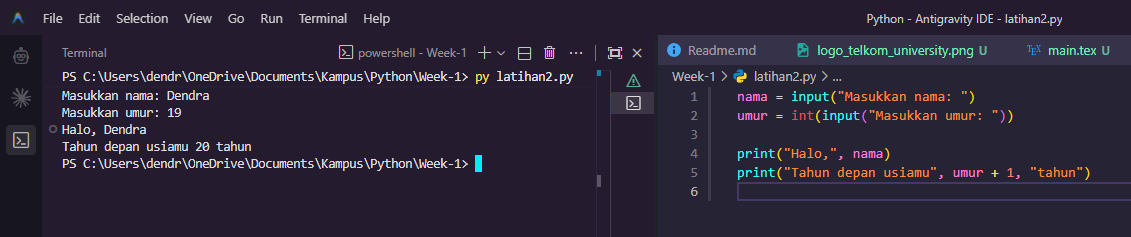
\includegraphics[width=0.85\textwidth]{image/latihan2.png}%
    }{%
        \imageplaceholder{Output Percobaan 2: Input Pengguna dan Konversi Tipe}%
    }
    \caption{Hasil/Output Percobaan 2: Input Pengguna dan Konversi Tipe}
\end{figure}

\subsubsection{Analisis}
Percobaan 2 menggarisbawahi karakteristik utama fungsi \texttt{input()} di Python 3, yaitu selalu mengembalikan data masukan pengguna dalam format bertipe \texttt{str} (string). Konsekuensinya, jika masukan angka usia tidak dikonversi secara eksplisit dan langsung dioperasikan dengan perintah $umur + 1$, interpreter akan menghentikan eksekusi program dengan galat fatal \texttt{TypeError: can only concatenate str (not "int") to str}.

Penerapan *type casting* melalui pembungkusan fungsi \texttt{int(input(...))} secara sukses mengubah representasi string menjadi bilangan bulat biner sehingga operasi penambahan aritmatika dapat berjalan dengan benar. Apabila masukan nama berupa \texttt{"Dimas"} dan usia \texttt{19}, kalkulasi $19 + 1$ secara deterministik menghasilkan angka 20 yang ditampilkan secara natural pada kalimat keluaran.

\subsection{Percobaan 3: Percabangan if-else Bilangan Ganjil/Genap}
\subsubsection{Algoritma}
\begin{enumerate}
    \item Mulai program.
    \item Baca masukan bilangan integer dari konsol dan simpan ke variabel \texttt{angka}.
    \item Lakukan pengujian kondisi percabangan biner: uji apakah sisa hasil bagi \texttt{angka} dengan 2 sama dengan 0 (\texttt{angka \% 2 == 0}).
    \begin{enumerate}[label=\alph*.]
        \item Jika bernilai benar (\textit{True}), jalankan blok \texttt{if}: cetak \texttt{"[angka] adalah bilangan genap"}.
        \item Jika bernilai salah (\textit{False}), jalankan blok \texttt{else}: cetak \texttt{"[angka] adalah bilangan ganjil"}.
    \end{enumerate}
    \item Selesai.
\end{enumerate}

\subsubsection{Hasil / Output}
\begin{figure}[H]
    \centering
    \IfFileExists{image/latihan3.png}{%
        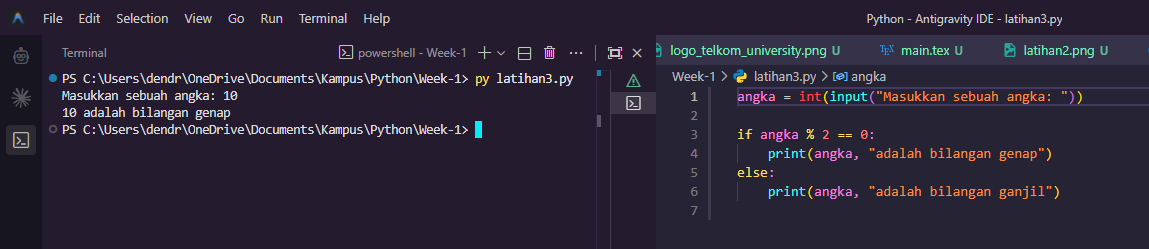
\includegraphics[width=0.85\textwidth]{image/latihan3.png}%
    }{%
        \imageplaceholder{Output Percobaan 3: Percabangan if-else Genap Ganjil}%
    }
    \caption{Hasil/Output Percobaan 3: Percabangan if-else Genap Ganjil}
\end{figure}

\subsubsection{Analisis}
Percobaan 3 mengimplementasikan struktur kontrol percabangan dua arah (\textit{binary decision}). Operator aritmatika modulo (\texttt{\%}) bertindak sebagai penentu kondisi logika dengan menghitung sisa pembagian bulat. Secara matematis, bilangan bulat $k$ memenuhi $k \equiv 0 \pmod 2$ jika dan hanya jika $k$ genap, serta $k \equiv 1 \pmod 2$ jika $k$ ganjil.

Ekspresi relasional \texttt{angka \% 2 == 0} menghasilkan nilai boolean murni (\texttt{True} atau \texttt{False}). Ketika diuji dengan angka 12, operasi $12 \pmod 2$ menghasilkan nilai 0 sehingga kondisi perbandingan bernilai \texttt{True} dan blok pernyataan \texttt{if} dieksekusi. Sebaliknya, jika diuji dengan angka 7, operasi $7 \pmod 2$ menghasilkan 1 ($1 == 0 \to \text{False}$), sehingga alur dialihkan ke blok penanganan alternatif \texttt{else}.

\subsection{Percobaan 4: Percabangan if-elif-else Kategori Nilai}
\subsubsection{Algoritma}
\begin{enumerate}
    \item Mulai program.
    \item Baca masukan nilai ujian bertipe integer ke dalam variabel \texttt{nilai}.
    \item Evaluasi kondisi berantai:
    \begin{enumerate}[label=\alph*.]
        \item Jika $nilai \ge 85$, simpan string \texttt{"A"} ke variabel \texttt{kategori}.
        \item Jika kondisi pertama salah dan $nilai \ge 70$, simpan string \texttt{"B"} ke variabel \texttt{kategori}.
        \item Jika kondisi kedua salah dan $nilai \ge 55$, simpan string \texttt{"C"} ke variabel \texttt{kategori}.
        \item Jika seluruh kondisi di atas salah, simpan string \texttt{"D"} ke variabel \texttt{kategori}.
    \end{enumerate}
    \item Tampilkan nilai kategori yang diperoleh: \texttt{"Kategori nilai kamu: [kategori]"}.
    \item Selesai.
\end{enumerate}

\subsubsection{Hasil / Output}
\begin{figure}[H]
    \centering
    \IfFileExists{image/latihan4.png}{%
        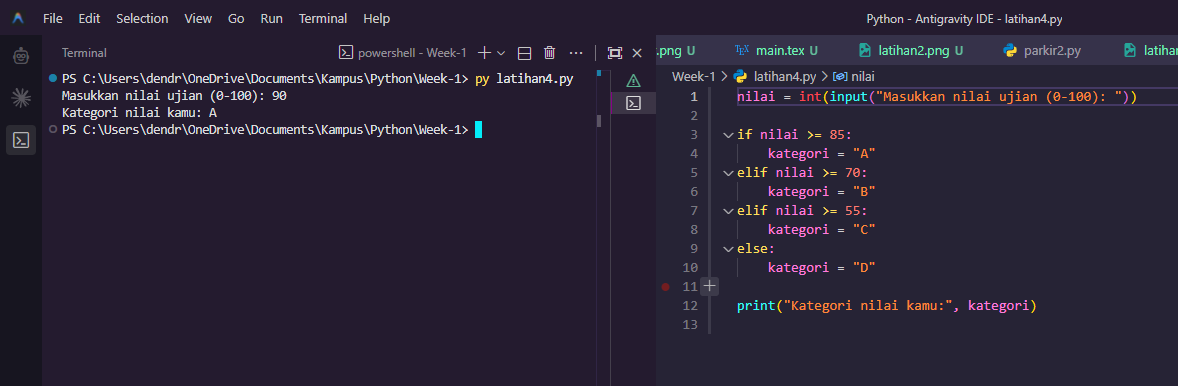
\includegraphics[width=0.85\textwidth]{image/latihan4.png}%
    }{%
        \imageplaceholder{Output Percobaan 4: Percabangan if-elif-else Kategori Nilai}%
    }
    \caption{Hasil/Output Percobaan 4: Percabangan if-elif-else Kategori Nilai}
\end{figure}

\subsubsection{Analisis}
Percobaan 4 memperlihatkan pemanfaatan struktur seleksi jamak (\textit{multi-way branching}) menggunakan kombinasi \texttt{if-elif-else}. Mekanisme kerja struktur ini bersifat sekuensial dan menerapkan evaluasi pemutusan dini (\textit{short-circuit evaluation}), di mana evaluasi kondisi berhenti seketika saat satu kondisi pertama bernilai \texttt{True}.

Oleh sebab itu, penyusunan kondisi dari nilai ambang batas tertinggi ke terendah ($85 \to 70 \to 55$) merupakan keharusan mutlak. Jika urutannya dibalik (misalnya memeriksa $nilai \ge 55$ paling awal), maka nilai tinggi seperti 90 akan langsung terperangkap pada kondisi pertama dan secara keliru dikategorikan sebagai C. Pada pengujian dengan nilai masukan 78, kondisi pertama ($78 \ge 85$) bernilai \texttt{False}, alur lanjut ke klausa kedua ($78 \ge 70$) yang bernilai \texttt{True}, sehingga variabel \texttt{kategori} terisi \texttt{"B"} dan blok evaluasi di bawahnya langsung dilewati.

\subsection{Percobaan 5: Studi Kasus Cek Kelulusan Mahasiswa}
\subsubsection{Algoritma}
\begin{enumerate}
    \item Mulai program.
    \item Baca string nama mahasiswa dari pengguna dan simpan ke variabel \texttt{nama}.
    \item Baca nilai akhir mahasiswa, ubah menjadi integer, dan simpan ke variabel \texttt{nilai}.
    \item Uji kelulusan: jika $nilai \ge 60$, tetapkan $status = \text{"LULUS"}$; selain itu tetapkan $status = \text{"TIDAK LULUS"}$.
    \item Tampilkan kalimat status kelulusan mahasiswa menggunakan format f-string.
    \item Uji grade huruf:
    \begin{enumerate}[label=\alph*.]
        \item Jika $nilai \ge 85$, tetapkan $grade = \text{"A"}$.
        \item Jika $nilai \ge 70$, tetapkan $grade = \text{"B"}$.
        \item Jika $nilai \ge 55$, tetapkan $grade = \text{"C"}$.
        \item Jika kondisi di atas tidak terpenuhi, tetapkan $grade = \text{"D"}$.
    \end{enumerate}
    \item Tampilkan teks \texttt{"Grade: "} diikuti nilai variabel \texttt{grade}.
    \item Selesai.
\end{enumerate}

\subsubsection{Hasil / Output}
\begin{figure}[H]
    \centering
    \IfFileExists{image/studi_kasus.png}{%
        \includegraphics[width=0.85\textwidth]{image/studi_kasus.png}%
    }{%
        \IfFileExists{image/latihan5.png}{%
            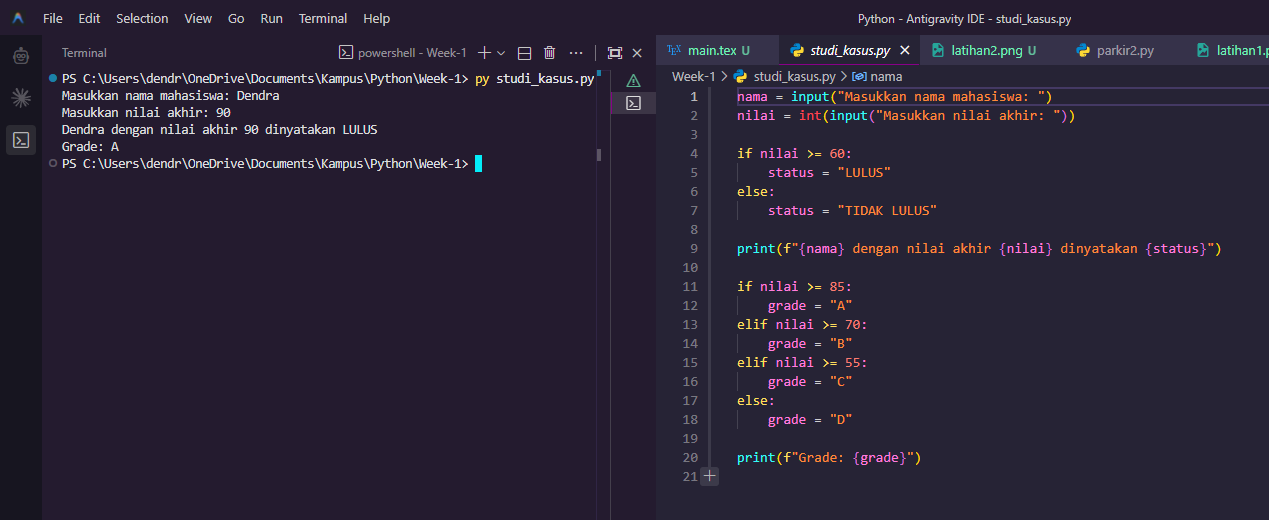
\includegraphics[width=0.85\textwidth]{image/latihan5.png}%
        }{%
            \imageplaceholder{Output Percobaan 5: Studi Kasus Cek Kelulusan Mahasiswa}%
        }%
    }
    \caption{Hasil/Output Percobaan 5: Studi Kasus Cek Kelulusan Mahasiswa}
\end{figure}

\subsubsection{Analisis}
Percobaan 5 memadukan seluruh konsep dasar yang dipelajari pada Modul 1 ke dalam program evaluasi terpadu. Terdapat dua blok percabangan independen: blok pertama menangani evaluasi biner status kelulusan berdasarkan aturan ambang kelulusan akademik ($\ge 60$), sedangkan blok kedua menangani klasifikasi bertingkat huruf mutu A--D.

Program memanfaatkan fitur \textit{formatted string literals} (f-string: \texttt{f"\{nama\}..."}) yang diperkenalkan sejak Python 3.6. f-string memungkinkan interpolasi ekspresi variabel secara langsung dan ekspresif di dalam string tanpa membutuhkan konkatenasi berulang atau konversi tipe string manual. Pada pengujian masukan dengan data uji nama \texttt{"Sinta"} dan nilai akhir \texttt{72}, blok kelulusan menetapkan status \texttt{LULUS} ($72 \ge 60$), dan blok grade menetapkan nilai huruf \texttt{B} ($70 \le 72 < 85$). Keduanya dicetak secara berurutan dan menghasilkan informasi akademik yang utuh dan akurat.

% ============================================================
% KESIMPULAN
% ============================================================
\section{KESIMPULAN}
Berdasarkan serangkaian percobaan yang telah dilakukan pada Praktikum Modul 1, dapat ditarik beberapa kesimpulan penting sebagai berikut:
\begin{enumerate}
    \item Python mengimplementasikan sistem pengetikan data dinamis (\textit{dynamically typed}), di mana alokasi tipe data untuk setiap variabel ditentukan secara otomatis pada saat inisialisasi nilai tanpa memerlukan deklarasi tipe secara statis. Fungsi bawaan \texttt{type()} efektif digunakan untuk memverifikasi kelas tipe data dari variabel yang dibuat.
    \item Fungsi pembacaan masukan konsol \texttt{input()} selalu mengembalikan data dengan representasi bertipe string (\texttt{str}). Untuk melakukan pemrosesan matematis dan evaluasi komparasi numerik, diperlukan konversi tipe eksplisit (\textit{type casting}) ke format \texttt{int} atau \texttt{float} guna menghindari galat \texttt{TypeError}.
    \item Struktur kontrol percabangan \texttt{if-else} dan \texttt{if-elif-else} memungkinkan algoritma mengambil keputusan logis secara fleksibel berdasarkan evaluasi ekspresi kondisi Boolean. Python menerapkan aturan indentasi spasi yang ketat sebagai pengganti kurung kurawal pembatas blok instruksi.
    \item Pada struktur percabangan berantai \texttt{if-elif-else}, urutan pemeriksaan kondisi dari nilai batas tertinggi menuju terendah sangat krusial karena mekanisme evaluasi berjalan secara sekuensial dari atas ke bawah dan menghentikan evaluasi begitu kondisi pertama bernilai benar (\textit{short-circuit evaluation}).
    \item Pemanfaatan f-string (\textit{formatted string literals}) pada Python mempermudah penggabungan berbagai tipe data ke dalam satu kalimat keluaran yang terstruktur dan rapi pada antarmuka konsol.
\end{enumerate}

% ============================================================
% DAFTAR PUSTAKA
% ============================================================
\section{DAFTAR PUSTAKA}

\begin{enumerate}
    \item Tim Dosen Algoritma dan Pemrograman. (2025). \textit{Modul Praktikum 1: Variabel, Tipe Data, dan Struktur Kontrol Percabangan}. Program Studi S1 Sistem Informasi, Fakultas Rekayasa Industri, Telkom University Surabaya.

    \item Python Software Foundation. (2024). \textit{Built-in Types and Control Flow Tools Documentation (Python 3.12)}. Diakses dari \url{https://docs.python.org/3/}.

    \item Van Rossum, G., \& Drake, F. L. (2009). \textit{Python 3 Reference Manual}. CreateSpace Independent Publishing Platform.
\end{enumerate}

\end{document}
